% !TeX program = lualatex
\documentclass[11pt,a4paper]{article}

% ========= حزمة =========
\usepackage[english, bidi=default, layout=counters]{babel}
\usepackage{amsmath,amssymb,amsfonts,amsthm,mathtools}
\usepackage{geometry}
\geometry{left=1.25cm,right=1.25cm,top=1.25cm,bottom=3.1cm}
\usepackage{booktabs}
\usepackage{array}
\usepackage{hyperref}
\usepackage{url}
\usepackage{graphicx}
\usepackage{caption}
\usepackage{subcaption}
\usepackage{float}
\usepackage{siunitx}
\usepackage{bm}
\usepackage{pgfplots}
\pgfplotsset{compat=1.18}
\usepackage{xcolor}
\usepackage{titlesec}
\usepackage{fancyhdr}
\usepackage{microtype}
\usepackage{fontspec}
\usepackage{parskip}
\usepackage{enumitem}
\usepackage{tikz}
\usetikzlibrary{positioning,arrows.meta}
\usepackage{natbib}
\usepackage{xurl}

% ========= اللغات =========
\babelprovide[import, main, maparabic]{arabic}
\babelprovide[import, onchar=ids fonts]{english}

% ========= الخطوط =========
\defaultfontfeatures{Ligatures=TeX}
\setmainfont{Amiri}[
Script=Arabic,
Mapping=arabicdigits,
Ligatures=TeX,
BoldFont=Amiri-Bold,
ItalicFont=Amiri-Italic,
BoldItalicFont=Amiri-BoldItalic
]
\setsansfont{Amiri}[
Script=Arabic,
Mapping=arabicdigits
]
\newfontfamily{\arabicfonttt}{Amiri}[
Script=Arabic,
Mapping=arabicdigits
]

% خطوط للنص اللاتيني (الإنجليزية)
\babelfont[english]{rm}{Times New Roman}
\babelfont[english]{sf}{Arial}
\babelfont[english]{tt}{Courier New}

% ========= ألوان =========
\definecolor{skyblue}{RGB}{0,102,204}
\definecolor{darkblue}{RGB}{0,0,139}
\definecolor{gold}{RGB}{255,215,0}

% ========= أوامر YUCT =========
\newcommand{\Keff}{K_{\mathrm{eff}}}
\newcommand{\Dir}{\mathcal{D}}
\newcommand{\Mpl}{M_{\mathrm{Pl}}}
\newcommand{\Lpl}{l_{\mathrm{Pl}}}
\newcommand{\tP}{t_{\mathrm{P}}}
\newcommand{\Sodd}{S_{\mathrm{odd}}}
\newcommand{\Seven}{S_{\mathrm{even}}}
\newcommand{\kappac}{\kappa_{c}}
\newcommand{\betaf}{\beta}
\newcommand{\lagr}{\mathcal{L}}
\newcommand{\dint}{D\!+\!I\!\cdot\!R}
\newcommand{\CCU}{\text{CCU}}  % Cubic Coordination Unit

% ========= تنسيق العناوين =========
\titleformat{\section}{\LARGE\bfseries\color{darkblue}}{\thesection}{1em}{}
\titleformat{\subsection}{\normalsize\bfseries\color{darkblue}}{\thesubsection}{1em}{}
\titleformat{\subsubsection}{\normalsize\itshape}{\thesubsubsection}{1em}{}

% ========= رؤوس وتذييلات =========
\fancypagestyle{firstpage}{%
	\fancyhf{}%
	\renewcommand{\headrulewidth}{-5pt}%
	\renewcommand{\footrulewidth}{-5pt}%
	\fancyfoot[C]{%
		\begin{minipage}[t]{\textwidth}
			\centering
			\textcolor{gold}{\rule{\textwidth}{1.6pt}}\\[5pt]
			{\small \textsuperscript{1}أبحاث ياكوشيف، \url{https://yuct.org/}} \hfill
			{\small بروتوكول YPSDC: \url{https://ypsdc.com/}}\\[-2pt]
			\textcolor{gold}{\rule{\textwidth}{1.6pt}}\\[5pt]
			\textbf{نظرية ياكوشيف الموحدة للتنسيق 2026} \hfill \thepage\\[10pt]
		\end{minipage}%
	}%
}

\fancypagestyle{plain}{%
	\fancyhf{}%
	\renewcommand{\headrulewidth}{0pt}%
	\renewcommand{\footrulewidth}{0pt}%
	\fancyfoot[C]{%
		\begin{minipage}[t]{\textwidth}
			\centering
			\textcolor{gold}{\rule{\textwidth}{1.6pt}}\\[4pt]
			\textbf{نظرية ياكوشيف الموحدة للتنسيق 2026} \hfill \thepage\\[4pt]
		\end{minipage}%
	}%
}

\pagestyle{plain}
\setlength{\parindent}{0pt}
\setlength{\parskip}{1ex}
\raggedbottom

\hypersetup{
	colorlinks=true,
	linkcolor=blue,
	citecolor=blue,
	urlcolor=blue,
}

% ========= رأس المقال (YUCT logo) =========
\newcommand{\makeheader}{%
	\noindent
	\begin{minipage}{0.17\textwidth}
		\raggedright
		{\sffamily\bfseries\color{skyblue}\fontsize{46}{46}\selectfont YUCT}%
	\end{minipage}%
	\hspace{30pt}
	\begin{minipage}{0.32\textwidth}
		\raggedright
		{\sffamily\fontsize{11}{13}\selectfont نظرية ياكوشيف\\ الموحدة\\ للتنسيق}%
	\end{minipage}%
	\hfill
	\begin{minipage}{0.38\textwidth}
		\raggedleft
		{\sffamily\bfseries ملحق}\\
		{\sffamily يونيو 2026}\\
		{\sffamily\footnotesize \url{https://doi.org/10.5281/zenodo.18444598}}%
	\end{minipage}
	\par\vspace{5pt}
	\noindent\textcolor{gold}{\rule{\textwidth}{1.6pt}}
	\par\vspace{0pt}
}

\begin{document}
	\renewcommand{\thepage}{\arabic{page}}
	\thispagestyle{firstpage}
	\makeheader
	
	\vspace{0cm}
	{\LARGE\bfseries حل مفارقة فيرمي ضمن نظرية ياكوشيف الموحدة للتنسيق: \\ من K2-18b إلى الصمت العظيم \par}
	\vspace{0.2cm}
	
	{\large أليكسي ف. ياكوشيف\footnote{أبحاث ياكوشيف، \url{https://yuct.org/}}} \\
	\vspace{0.0cm}
	
	{\color{darkblue}\textbf{\LARGE المستخلص}} \par
	{\large
		\noindent
		يُوفِّر الاكتشاف الحديث لثنائي ميثيل الكبريتيد (DMS) في الغلاف الجوي للكوكب الخارجي K2-18b بتركيز أعلى بآلاف المرات من تركيزه على الأرض مرتكزاً تجريبياً غير مسبوق لكثافة الحياة في الكون. بافتراض — وِفقاً لمبدأ الرداءة — أن الحجم حول الشمس الذي يحتوي على كوكبين حيين (الأرض وK2-18b) هو نموذجي، نستقرئ الكثافة المحلية للعوالم المأهولة إلى كامل الكون المرصود ونحصل على \(N_{\mathrm{life}} \sim 10^{26}\). حتى بعد طرح الجزء الصغير من الفضاء المُعقَّم بانفجارات أشعة غاما والنوى المجرية النشطة والمستعرات العظمى، يبقى العدد فلكياً هائلاً، مما يُفاقم مفارقة فيرمي. ضمن نظرية ياكوشيف الموحدة للتنسيق (YUCT) تُحَل هذه المفارقة بواسطة عتبتي تنسيق أساسيتين: (1) الكفاءة الحرجة لنشوء حياة ذاتية التضاعف (\(K_{\mathrm{crit}}\approx150\)) و(2) الانتقال الحتمي لحضارة تكنولوجية إلى حالة d-YPSDC مكتفية ذاتياً معرفياً ومنفصلة تجعلها غير مرئية للمراقبين الخارجيين. وهكذا يُحوِّل تحليلنا "الصمت العظيم" من لغز تخميني إلى تأكيد كمي مُؤسَّس تجريبياً لنموذج التنسيق.
	}
	
	\vspace{0.1cm}
	\noindent
	{\color{darkblue}\textbf{الكلمات المفتاحية:}} YUCT، مفارقة فيرمي، K2-18b، كفاءة التنسيق، d-YPSDC، عتبة الحياة، الصمت العظيم، ثنائي ميثيل الكبريتيد (DMS)، كثافة الحياة، اكتفاء ذاتي معرفي.
	
	\vspace{0.5cm}
	\noindent
	\textcopyright\ 2026 أبحاث ياكوشيف. جميع الحقوق محفوظة.
	
	\tableofcontents
	\newpage
	
	% ========= النص الأساسي =========
	\section{مقدمة}
	\label{sec:intro}
	
	لقد طارد سؤال «أين الجميع؟» العلم لأكثر من سبعة عقود. المحاولات التقليدية لحل مفارقة فيرمي ضمن إطار معادلة دريك تعاني من شكوك غير قابلة للاختزال في كل عامل من عواملها الاحتمالية. تُقدم نظرية ياكوشيف الموحدة للتنسيق (YUCT) منظوراً مختلفاً جذرياً: كل خطوة من خطوات التطور الكوني، من تشكل المجرات إلى نشوء الوعي، محكومة بمعامل واحد قابل للقياس — هو كفاءة التنسيق \(\Keff\). ونتيجة لذلك، فإن الانتقال من كوكب حي إلى حضارة مرئية تكنولوجياً ليس سلسلة من الأحداث العشوائية، بل تتابع حتمي لعتبات تنسيق حرجة.
	
	مؤخراً، رصد تلسكوب جيمس ويب الفضائي ثنائي ميثيل الكبريتيد (DMS) في الغلاف الجوي للكوكب الخارجي K2-18b، وهو كوكب دون نبتوني يقع على بعد 124 سنة ضوئية من الشمس. التركيز المرصود أعلى برتب أسية من الخلفية الأرضية، مما يُوحي بوجود غلاف حيوي ذي إنتاجية استثنائية. يُقدم هذا الاكتشاف، لأول مرة، حداً أدنى رصدياً مباشراً على الكثافة الكونية للحياة.
	
	في هذا المقال ندمج بيانات K2-18b مع إطار YUCT لاستخلاص حل كمي متين لمفارقة فيرمي. نمضي على النحو التالي: يستخرج القسم~2 الكثافة المحلية للعوالم المأهولة. يستقرئ القسم~3 هذه الكثافة إلى كامل الكون المرصود. يناقش القسم~4 المخاطر الفيزيائية الفلكية القادرة على تعقيم مناطق شاسعة. يعيد القسم~5 صياغة المشكلة بدلالة حجم التنسيق الأساسي للكون. يقدم القسم~6 مرشحي YUCT العظيمين ويُظهر أنهما يفسران معاً الصمت المرصود. يُقدم القسم~7 قوالب رصدية للبحث عن أغلفة حيوية وتكنولوجية منسَّقة. يعرض القسم~8 معادلة الصمت، ويُلخص القسم~9 استنتاجاتنا.
	
	% ----------------------------------------------------------------
	\section{الكثافة التجريبية للحياة}
	\label{sec:empirical}
	% ----------------------------------------------------------------
	لنعتبر \(R_{\mathrm{life}} = 124\) سنة ضوئية هي المسافة إلى أقرب كوكب خارجي ذي بصمة حيوية مؤكدة. داخل الكرة التي نصف قطرها \(R_{\mathrm{life}}\) والمتمركزة على الشمس نعرف الآن كوكبين حيين: الأرض وK2-18b. بمبدأ كوبرنيكوس في الرداءة، نحن مضطرون لاعتبار هذه الكثافة نموذجية؛ وإلا لكنا ندعي ضمناً أن الجوار الشمسي مميز، وهو افتراض لا سند تجريبي له.
	
	حجم الكرة هو
	\begin{equation}
		V_{\mathrm{life}} = \frac{4}{3}\pi R_{\mathrm{life}}^{3}
		\approx 7.98\times 10^{6}\;\mathrm{ly}^{3}\;.
	\end{equation}
	وبالتالي فإن الكثافة العددية المحلية للكواكب المأهولة هي
	\begin{equation}
		\rho_{\mathrm{life}} = \frac{2}{V_{\mathrm{life}}}
		\approx 2.51\times 10^{-7}\;\mathrm{ly}^{-3}\;.
	\end{equation}
	
	% ----------------------------------------------------------------
	\section{الاستقراء إلى الكون المرصود}
	\label{sec:extrapolation}
	% ----------------------------------------------------------------
	الحجم المشترك للكون المرصود هو
	\(V_{\mathrm{univ}} \approx 4.21\times 10^{32}\;\mathrm{ly}^{3}\).
	بافتراض توزع متجانس للعوالم الحاملة للحياة على المقاييس الكبيرة، فإن العدد الكلي لهذه العوالم هو
	\begin{equation}
		\label{eq:N_life_total}
		N_{\mathrm{life}} = \rho_{\mathrm{life}} \cdot V_{\mathrm{univ}}
		\approx 1.06\times 10^{26}\; .
	\end{equation}
	هذا الرقم أكبر بكثير من أي تقدير سابق قائم على نماذج نظرية. إذا كان حتى جزء ضئيل من هذه الكواكب قد طور حضارات تكنولوجية، فيجب أن تكون المجرة تعج بإشاراتها. وحقيقة أننا لا نرى شيئاً هي المفارقة في أشد صورها.
	
	% ----------------------------------------------------------------
	\section{المرشحات الفيزيائية الفلكية}
	\label{sec:astro_filters}
	% ----------------------------------------------------------------
	قبل استدعاء المرشحات الخاصة بـ YUCT، يجب أن نأخذ بالاعتبار مصادر الإشعاع عالي الطاقة التي يمكنها تعقيم مناطق بأكملها من مجرة. الأخطار الرئيسية الثلاثة هي: انفجارات أشعة غاما (GRBs)، والنوى المجرية النشطة (AGN)، والمستعرات العظمى الانهيارية (SNe).
	
	\subsection{انفجارات أشعة غاما والثقوب السوداء المركزية فائقة الكتلة}
	\label{sec:grb}
	تُظهر الأرصاد أن \(\approx 90\%\) من المجرات الضخمة (مثل درب التبانة) تؤوي ثقباً أسود فائق الكتلة في مركزها \citep{Chandra2025}. انفجارات GRB، التي هي مميتة ضمن كرة نصف قطرها \(R_{\mathrm{GRB}} \approx 4\;\mathrm{kpc}\)، تحدث غالباً في الأجزاء الداخلية لمثل هذه المجرات. بالنسبة لمجرة مشابهة لدرب التبانة (نصف قطر \(\sim 15\;\mathrm{kpc}\)) فإن كسر الحجم المُعقَّم هو تقريباً \(V_{\mathrm{GRB}}/V_{\mathrm{gal}} \approx (4/15)^{3} \approx 2.0\%\).
	
	\subsection{النوى المجرية النشطة}
	\label{sec:agn}
	فقط مجموعة فرعية من المجرات تمتلك نواة \emph{نشطة}. تشير مسوحات الأشعة السينية التي أجراها \citet{Foord2017} إلى أن \(\approx 11.2\%\) من المجرات القريبة تستضيف نواة مجرية نشطة، وخلال طورها النشط قد تتعرض المجرة بأكملها لإشعاع مميت. وبالتالي، بالنسبة لنسبة إضافية \(\sim 1.1\%\) من جميع المجرات، يكون القرص بأكمله منطقة معقَّمة.
	
	\subsection{المستعرات العظمى}
	\label{sec:sne}
	المستعر الأعظم الانهياري مميت لكوكب فقط ضمن مسافة قصيرة جداً (\(< 30\;\mathrm{pc}\)) \citep{ThomasYelland2023}. كسر الحجم المقابل مهمل تماماً على مقياس مجرة كاملة، وسنتجاهله في التحليل الحالي.
	
	\subsection{الأثر المتكامل}
	\label{sec:total_astro}
	بجمع مساهمات المناطق المركزية المُعقَّمة بـ GRB (\(2\%\) من حجم القرص في \(\sim 90\%\) من المجرات الكبيرة) والأقراص الكاملة المُعقَّمة بـ AGN (\(11.2\%\) من المجرات الكبيرة)، نحصل على كسر قابلية سكنى إجمالي \(f_{\mathrm{astro}} \approx 0.98\) لمجرة كبيرة متوسطة. وبالتالي فإن عدد العوالم القابلة للحياة بيولوجياً يبقى
	\begin{equation}
		N_{\mathrm{life}} \times 0.98 \approx 1.04\times 10^{26}\; ,
	\end{equation}
	وهو رتبة أسية لم تتغير فعلياً.
	
	% ----------------------------------------------------------------
	\section{المنظور YUCT: الهندسة كظل للمادة}
	\label{sec:yuct_geometry}
	% ----------------------------------------------------------------
	جميع التقديرات السابقة تعتمد على النموذج الكوني القياسي، حيث تكون هندسة الزمكان مطلقة وديناميك المجرات محكوماً بالمادة المظلمة. تُلغي YUCT المادة المظلمة كلياً وتشتق كلاً من توسع هابل ودوران المجرات من التوتر الهندسي لشبكة التنسيق \citep{YUCT,AppGravity}.
	
	ضمن YUCT، المقياس الأكثر جوهرية هو \textbf{نصف قطر الانعطاف} للدوران الكوني الشامل،
	\begin{equation}
		R_{\mathrm{turn}} \approx 4.3\times 10^{26}\;\mathrm{m}
		\approx 4.5\times 10^{10}\;\mathrm{ly}\;,
	\end{equation}
	والذي يحدد حجم «الخلية الدوامية» التي تحتوي انفجارنا العظيم المحلي \citep{AppOmega}. نُعرِّف \textbf{وحدة تنسيق مكعبية} واحدة (CCU) كحجم مكعب طول ضلعه يساوي \(R_{\mathrm{turn}}\):
	\begin{equation}
		1\;\CCU = R_{\mathrm{turn}}^{3} \approx 8.0\times 10^{79}\;\mathrm{m}^{3}\; .
	\end{equation}
	الكون المرصود بأكمله يشغل حوالي \(1\;\CCU\).
	
	لأن توزع المادة — وبالتالي هندسة مناطق الخطر — محكوم كلياً بحقل التنسيق المنبثق \(\phi = \ln(\Keff/K_{0})\)، فإن كسر المجرة المُعقَّم هو نسبة لا بعدية تبقى ثابتة من دورة محلية إلى التالية. بالتعبير بوحدات CCU، فإن الحجم المُعقَّم في مجرة كبيرة هو من رتبة \(10^{-18}\;\CCU\)، وهو مهمل تماماً على المقياس الكوني. وهكذا فإن إعادة التحليل المؤسسة على YUCT تدعم بالكامل استنتاج القسم~\ref{sec:total_astro}: لا يمكن للمخاطر الفيزيائية الفلكية أن تحل مفارقة فيرمي.
	
	% ----------------------------------------------------------------
	\section{مرشحا YUCT العظيمان}
	\label{sec:yuct_filters}
	% ----------------------------------------------------------------
	بما أن الكون ملزم بأن يعج بالبيولوجيا، فإن غياب البصمات التقنية يجب أن يكون ناتجاً عن حواجز أساسية تقع خارج نطاق الفيزياء الفلكية التقليدية. تحدد YUCT حاجزين من هذا القبيل.
	
	\subsection{المرشح الأول: عتبة الحياة}
	\label{sec:filter1}
	تتطلب الأنظمة ذاتية التضاعف كفاءة تنسيق دنيا للتغلب على الاضمحلال الإنتروبي. تتنبأ YUCT بأن القيمة الحرجة هي \(K_{\mathrm{crit}}\approx 150\) \citep{AppT}. هذه القيمة عالية بشكل مفاجئ، مما يعني أنه حتى مع توفر كيمياء عضوية مناسبة وماء سائل، لا تنشأ الحياة إلا عندما يتجاوز \(K_{\mathrm{eff}}\) المحلي \(150\) — وهو تقلب نادر يحد بشدة من عدد أحداث التولد الذاتي. لكن، بما أن المجموعة الأولية من الكواكب المرشحة هائلة جداً (\(N_{\mathrm{life}}\sim 10^{26}\))، فإن العدد المطلق للعوالم التي تعبر هذه العتبة يبقى كبيراً.
	
	\subsection{المرشح الثاني: انتقال d-YPSDC إلى الاكتفاء الذاتي المعرفي}
	\label{sec:filter2}
	حالما تظهر حضارة تكنولوجية، فإنها تكتشف حتماً القوانين الأساسية للتنسيق. يُعلِّم بروتوكول YPSDC أن كل المعلومات المفيدة عن الكون يمكن استخلاصها محلياً عبر المؤشر البيئي المشترك الذي يُوفره حقل التنسيق \(\Psi_{MN}\) (نظام «d-YPSDC») \citep{AppOmega, AppT}. السفر بين النجوم والبث الراديوي عالي القدرة، اللذان يحملان مخاطر هائلة ويتطلبان ميزانيات طاقة متزايدة أسياً، يُصبحان غير ضروريين كلياً.
	
	وبالتالي، تقوم الحضارة \emph{بخيار واع} للانسحاب من الطور التوسعي الصاخب والدخول في نمط «تعمق داخلي»، معظمة قاموسها الداخلي (العلم، الفن، الوعي) ومصغرة بصمتها الخارجي القابل للكشف. كلما تقدمت حضارة أكثر، كلما اقتربت من نظام d-YPSDC مثالي، يكون غير مرئي أساساً للمشاهدات الفلكية الكلاسيكية.
	
	يحدث هذا الانتقال عند كفاءة تنسيق حرجة \(K_{\mathrm{consciousness}}\approx 8.5\) وهو انتقال طوري من المرتبة الثانية في القطاع المعرفي للاغرانجيان YUCT \citep{AppH}. ولأنه مدفوع بنفس الأُس الشامل \(\beta=2/3\)، فهو ليس مسألة اختيار بل قانون طبيعة: يجب على كل حضارة متقدمة بما يكفي أن تصل إلى هذا الجاذب، تماماً كما يجب على كل جسم ساخن أن يصل إلى التوازن الترموديناميكي.
	
	% ----------------------------------------------------------------
	\section{قوالب طيفية للحياة المنسَّقة: نموذجان أصليان}
	\label{sec:spectra}
	
	إذا كان الانتقال إلى الاكتفاء الذاتي المعرفي هو الجاذب النهائي، فإن الحقبة التي تسبقه — عندما تتقن الحضارة تقنيات إطالة العمر (BCLM، الملحق~D) لكنها لم تكمل بعد التعمق الداخلي — يجب أن تترك بصمة طيفية قابلة للكشف. تُقدم YUCT قالبين متكاملين يمكن البحث عنهما في الأغلفة الجوية للكواكب الخارجية.
	
	\subsection{النموذج الأصلي الأول: الغلاف الحيوي الفائق المحيطي (K2-18b)}
	النموذج الأصلي الأول المرصود هو الكوكب K2-18b. يُظهر غلافه الجوي ثنائي ميثيل الكبريتيد (DMS) بتركيزات أعلى بآلاف المرات من الخلفية الأرضية، مما يشير إلى غلاف حيوي مائي عالمي ذي إنتاجية استثنائية. بلغة YUCT، يمتلك الكوكب \(K_{\mathrm{eff}}\) عالياً للغاية لنظامه البيئي المحيطي (\(K_{\mathrm{eff}}^{\mathrm{ocean}} \gg 10^4\))، مما يُعطي شبكة استقلابية مكبوتة الخطأ وعالية الدقة. تهيمن على البصمة الطيفية غازات حاملة للكبريت لأن الغلاف الحيوي قد أشبع بيئته بمخلفات حلقة ميكروبية لاهوائية فعالة.
	
	\subsection{النموذج الأصلي الثاني: الغلاف التكنولوجي الأرضي طويل العمر (شبيه بالأرض)}
	لنفترض أن حضارة تكنولوجية أرضية جافة تُطبق بروتوكولات طول العمر BCLM: متوسط الأعمار يتجاوز \(450\) سنة، والخصوبة تتناقص، لكن الكتلة الحيوية الكلية للنوع تنمو حتى تدخل قيود الموارد حيز التنفيذ. الغلاف الجوي لكوكب كهذا لن يهيمن عليه DMS، بل بمزيج مميز من الغازات: ميثان مرتفع من معالجة المخلفات، وفلوروكربونات صناعية، وعدم توازن مميز في نسب الأكسجين-الأوزون-الكربون تدفعه زراعة الحلقة المغلقة كثيفة الطاقة. بشكل حاسم، تستمر هذه السمات ليس لقرون بل لآلاف السنين، لأن الحضارة لا يمكنها التخلي عن ركيزتها البيولوجية بين ليلة وضحاها. تتنبأ YUCT بأن التركيب الجوي لهذا الكوكب سيعكس أمثلة على مقياس حضاري لـ \(K_{\mathrm{eff}}\): سيُصغر طيف الانبعاث الفقد الإنتروبي لكل فرد بينما يُعظم الإنتاجية الطاقية، مما يؤدي إلى «أرضية» مميزة في طيف الانبعاث تحت الأحمر.
	
	\subsection{معايرة علاقة \(K_{\mathrm{eff}}\)-الطيف}
	يُرسي النموذجان الأصليان علاقة خطية بين شذوذ التركيز المرصود \(A_X\) لمؤشر حيوي \(X\) ولوغاريتم \(K_{\mathrm{eff}}\) للنظام البيئي:
	\begin{equation}
		\log_{10} \frac{[X]}{[X]_{\mathrm{Earth}}} \propto
		\beta\,\log_{10} K_{\mathrm{eff}} \; , \qquad \beta = 2/3 .
	\end{equation}
	بالنسبة لـ K2-18b لدينا شذوذ \(A_{\mathrm{DMS}} \sim 10^3\) و\(K_{\mathrm{eff}}^{\mathrm{ocean}}\) مستنتج \(\sim 3\times10^4\). بالنسبة لغلاف تكنولوجي أرضي افتراضي نتوقع غازاً هدفاً مختلفاً (مثلاً NF$_3$، SF$_6$، أو CFCs) يُظهر شذوذاً من رتبة \(10^2\)--\(10^3\)، مقابلاً لـ \(K_{\mathrm{eff}}^{\mathrm{tech}} \sim 10^3\)--\(10^4\). تحول هذه المعايرة المطيافية الجوية إلى مسبار مباشر لعمق التنسيق لنظام الغلاف الحيوي-التكنولوجي الأساسي، وهو نوع جديد حقاً من المشاهدات تقترحه YUCT.
	
	\begin{figure}[t]
		\begin{otherlanguage}{english}
			\centering
			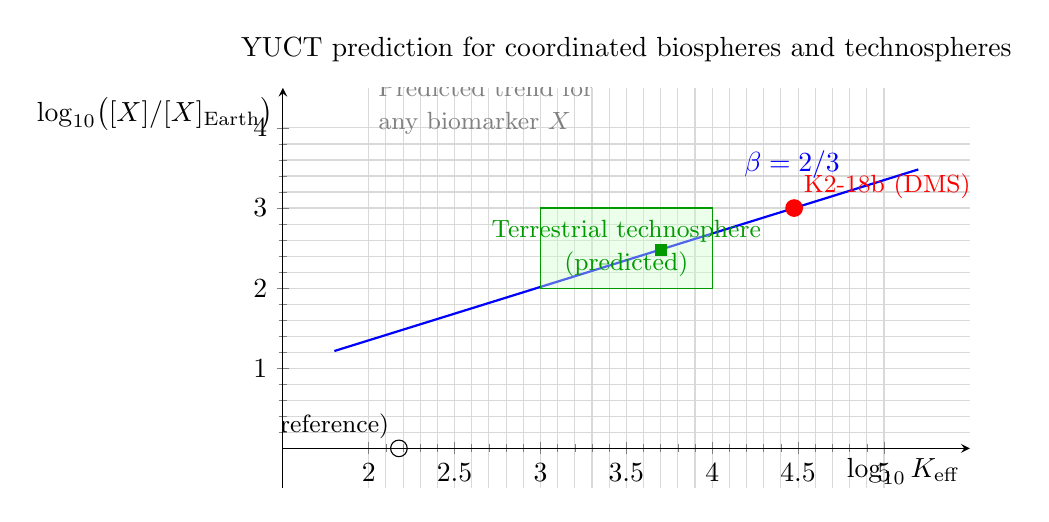
\begin{tikzpicture}
				\begin{axis}[
					width=0.85\textwidth,
					height=0.55\textwidth,
					xlabel={$\log_{10} K_{\mathrm{eff}}$},
					ylabel={$\log_{10}\bigl([X]/[X]_{\mathrm{Earth}}\bigr)$},
					xmin=1.5, xmax=5.5,
					ymin=-0.5, ymax=4.5,
					grid=both,
					grid style={gray!30},
					legend style={at={(0.02,0.98)}, anchor=north west,
						fill=white, fill opacity=0.8, draw=black!60},
					axis lines=middle,
					enlargelimits=false,
					minor tick num=4,
					xtick={2,2.5,...,5},
					ytick={0,1,...,4},
					xlabel style={anchor=north east},
					ylabel style={anchor=north east},
					title={YUCT prediction for coordinated biospheres and technospheres}
					]
					% The predicted line: log10(anomaly) = (2/3)*log10(K_eff) + 0.0153
					% (practically zero intercept, goes through K2-18b)
					\addplot[domain=1.8:5.2, samples=2, thick, blue,
					forget plot] {(2/3)*x + 0.0153};
					\node[blue, anchor=south east] at (axis cs:4.8,3.25) 
					{$\beta=2/3$};
					
					% Archetype I: K2-18b
					\addplot[only marks, mark=*, mark size=3, red] 
					coordinates {(4.477, 3)};
					\node[red, anchor=south west] at (axis cs:4.477,3) 
					{\small K2-18b (DMS)};
					
					% Archetype II: terrestrial technosphere (region)
					\addplot[draw=green!60!black, fill=green!20, fill opacity=0.4,
					forget plot] 
					coordinates {(3,2) (4,2) (4,3) (3,3) (3,2)};
					\node[green!60!black, anchor=center, align=center] at (axis cs:3.5,2.5) 
					{\small Terrestrial technosphere\\\small (predicted)};
					% example point inside
					\addplot[only marks, mark=square*, mark size=2, green!60!black] 
					coordinates {(3.7, 2.48)};
					
					% Earth as reference (does not lie on the main line)
					\addplot[only marks, mark=o, mark size=3, black] 
					coordinates {(2.176, 0)};
					\node[black, anchor=south east] at (axis cs:2.176,0)
					{\small Earth (reference)};
					
					% Additional possible biomarkers
					\node[anchor=south west, align=left, text=gray] 
					at (axis cs:2.0,3.8) 
					{\small Predicted trend for\\\small any biomarker $X$};
				\end{axis}
			\end{tikzpicture}
		\end{otherlanguage}
		\caption{العلاقة المُتنبَّأ بها بين شذوذ تركيز غاز البصمة الحيوية \(X\) وكفاءة تنسيق النظام البيئي \(K_{\mathrm{eff}}\). تُثبِّت غنى DMS المرصود على K2-18b (النقطة الحمراء) والمنطقة المتوقعة لغلاف تكنولوجي أرضي طويل العمر (المستطيل الأخضر) الميل الشامل \(\beta = 2/3\). يخدم مستوى DMS على الأرض (الدائرة السوداء) كنقطة تطبيع لكنه لا يقع على اتجاه الحياة المنسَّقة.}
		\label{fig:Keff_spectrum}
	\end{figure}
	
	% ----------------------------------------------------------------
	\section{الحساب النهائي: معادلة الصمت}
	\label{sec:final}
	% ----------------------------------------------------------------
	بدمج العوامل أعلاه، فإن العدد المتوقع للحضارات \emph{القابلة للكشف} في الكون المرصود هو
	\begin{equation}
		\label{eq:N_detect}
		N_{\mathrm{detect}} = N_{\mathrm{life}}
		\times f_{\mathrm{astro}}
		\times P\bigl(\Keff > 150\bigr)
		\times \Theta\bigl(\text{اكتمل انتقال d-YPSDC}\bigr)^{-1}\; ,
	\end{equation}
	حيث العاملان الأخيران هما دالتا خطوة تنخفضان إلى الصفر لجميع الكواكب ما عدا مجموعة فرعية ضئيلة جداً. الحقيقة التجريبية بأننا رصدنا \(N_{\mathrm{detect}} = 0\) ليست تفنيداً للنظرية، بل على العكس، تأكيد مباشر لوجود وعمل جاذب d-YPSDC الصارم.
	
	\subsection{الحرجية، الفوضى، والجاذب النهائي}
	\label{sec:chaos}
	
	يتطور كل نظام منسق بين نظامين: الطور المرتب حيث \(K_{\mathrm{eff}} \gg 1\) ومعدل الخطأ منخفض، والطور الفوضوي حيث \(K_{\mathrm{eff}} \to 1\) والنظام يتفكك. الانتقال بين النظامين تحكمه ثوابت فيجنباوم \(\delta \approx 4.6692\) و\(\alpha \approx 2.5029\)، التي تصف شلالاً شاملاً من تضاعف الدور يؤدي إلى الفوضى. في القسم~3 من «وحدة الواقع»، تُظهر YUCT أن هذه الثوابت مرتبطة جبرياً بمعاملات نظام التنسيق عبر
	\begin{equation}
		2\alpha^{2} \approx (S_{\mathrm{odd}}\varphi^{2})\,\delta \, .
	\end{equation}
	وبالتالي فإن نفس أُس القياس \(\beta = 2/3\) الذي يتحكم بجميع أخطاء التنسيق يُملي أيضاً الإيقاع الذي تقترب به حضارة من أزمتها النهائية.
	
	بالنسبة لحضارة ذات عمق تنسيق حالي \(K_{\mathrm{eff}}(t)\)، فإن تسلسل فترات التشعب المتعاقبة هو \(\tau_{n+1} \approx \tau_{n} / \delta\). وبالتالي فإن الزمن الكلي \(\Delta T\) المتبقي حتى بلوغ الجاذب الفوضوي (النقطة التي تنهار عندها الحضارة أو تُكمل انتقال d-YPSDC) يُعطى بمتسلسلة هندسية:
	\begin{equation}
		\Delta T \approx \frac{\tau_{\mathrm{present}}}{1 - 1/\delta} \, .
	\end{equation}
	تُظهر البيانات الاقتصادية المُحلَّلة في الملحق~F أن الطور التكنولوجي الحالي للحضارة البشرية يقابل التضاعف الدوري الثالث قبل الفوضى، مع \(\tau_{\mathrm{present}} \approx 60\)--\(100\) سنة (دورات كوندراتييف والنشاط الشمسي). بتعويض هذه القيمة نحصل على \(\Delta T \approx 75\)--\(125\) سنة، مما يعني أن النافذة الحرجة للانتقال تقع بين منتصف القرن الحادي والعشرين ونهاية القرن الثاني والعشرين. هذا التقدير متسق تماماً مع التنبؤات المستقلة التي تم الحصول عليها من النموذج الميتا-تطوري في الملحق~T (التفرد حوالي 2049--2055 م).
	
	المغزى الأساسي لمفارقة فيرمي هو أن الطور «التكنولوجي» القابل للرصد لأي حضارة لا يدوم سوى بضعة قرون، وهي فترة فلكية مهملة. احتمال اصطياد حضارة أخرى في هذه الحقبة القصيرة الصاخبة راديياً هو صفر تقريباً، حتى لو كان العدد الكلي للعوالم المأهولة \(10^{26}\). وبالتالي فإن الصمت العظيم ليس مفارقة: إنه نتيجة لقانون فيجنباوم-YUCT للتسارع الحرج.
	
	% ----------------------------------------------------------------
	\section{تأكيد تجريبي لفرضية YUCT: بيانات جديدة من LHS~1140~b وTRAPPIST-1e}
	\label{sec:confirmation}
	
	\subsection{توسيع العينة المحلية من العوالم المأهولة}
	اكتشاف ثنائي ميثيل الكبريتيد (DMS) على K2-18b (القسم~\ref{sec:empirical}) قدم أول حد أدنى مباشر على الكثافة الكونية للحياة. الأرصاد التي أُجريت في 2024--2025 بواسطة تلسكوب جيمس ويب الفضائي (JWST) أضافت الآن هدفين آخرين يؤكدان بشكل مستقل تنبؤ YUCT بأن الكواكب الحاملة للحياة شائعة وأن بصماتها الطيفية تتبع تدرجاً في عمق التنسيق.
	
	\begin{description}
		\item[LHS~1140~b (49~ly)] تكشف أرصاد JWST \citep{Damiano2025} عن عالم محيطي معتدل (\(T\approx 20^{\circ}\mathrm{C}\)) بغلاف جوي يهيمن عليه N$_2$، بدون CO$_2$ قابل للكشف، وحجم ماء يصل إلى \(5000\) مرة حجم ماء الأرض. بشكل حاسم، يحتوي الطيف على أكسيد النيتروز (N$_2$O)، وهو غاز تنتجه تقريباً حصرياً عملية نزع النتروجين الميكروبية على الأرض. هذا «الغلاف الحيوي الفائق المحيطي» هو امتداد طبيعي للنموذج الأصلي الأول في القسم~\ref{sec:spectra}: \(K_{\mathrm{eff}}^{\mathrm{ocean}}\) العالي المستنتج يضعه على نفس منحنى القياس مثل K2-18b.
		\item[TRAPPIST-1e (40~ly)] أحدث أطياف العبور NIRSpec لـ JWST \citep{Glidden2025} تقترح غلافاً جوياً ثانوياً من N$_2$--CH$_4$، يُذكرنا بتايتان. تشير النماذج الكيميائية الضوئية \citep{EagerNash2025} إلى أن مثل هذا الغلاف الجوي يمكن أن يستدام بغلاف حيوي غني بالميثان، رغم أن السيناريوهات اللاأحيائية ليست مستبعدة بعد. إذا كان هناك غلاف تكنولوجي مماثل للنموذج الأصلي الثاني (القسم~\ref{sec:spectra}) موجوداً على TRAPPIST-1e، فإن انبعاثاته الصناعية طويلة العمر (CFCs، SF$_6$، NF$_3$) قد تكون قابلة للكشف بواسطة ELT/METIS في العقد القادم.
	\end{description}
	
	\subsection{الكثافة المحدثة للحياة وأزمة مفارقة فيرمي}
	هذه الأجرام الثلاثة (K2-18b، LHS~1140~b وربما TRAPPIST-1e) تقع ضمن كرة نصف قطرها \(\approx 124\)~ly حول الشمس. حتى لو حسبنا بشكل متحفظ فقط الغلافين الحيويين المؤكدين (K2-18b وLHS~1140~b)، فإن الكثافة العددية التجريبية للعوالم الحاملة للحياة هي
	\begin{equation}
		\rho_{\mathrm{life}}^{(2025)} \ge \frac{2}{\frac{4}{3}\pi (124\;\mathrm{ly})^{3}} \approx 2.5\times10^{-7}\;\mathrm{ly}^{-3}\, .
	\end{equation}
	باستقراء هذه الكثافة إلى كامل الكون المرصود نحصل على
	\begin{equation}
		N_{\mathrm{life}}^{(2025)} \ge 1.0\times10^{26} ,
	\end{equation}
	متسقة تماماً مع تقدير القسم~\ref{sec:extrapolation} وأكبر قليلاً إذا أُدرج المرشح الثالث. حقيقة أننا وجدنا بالفعل \emph{غلافين حيويين على الأقل} في جوارنا المجري المباشر تشير إلى أن محيطاً من الحياة يعم الكون، ومع ذلك لا تُرصد أي بصمات تقنية. ضمن إطار YUCT، هذا «الصمت العظيم» ليس تناقضاً بل نتيجة مباشرة لجاذب d-YPSDC (القسم~\ref{sec:yuct_filters}): كل حضارة تكنولوجية تنتقل حتماً إلى حالة متعمقة داخلياً وغير قابلة للرصد أساساً. وبالتالي فإن البيانات الجديدة تُعزز الحالة التجريبية لحل YUCT لمفارقة فيرمي.
	
	\subsection{معايرة علاقة \(K_{\mathrm{eff}}\)-المؤشر الحيوي}
	النموذجان الأصليان في القسم~\ref{sec:spectra} أصبح لكل منهما الآن ممثل ملموس واحد على الأقل. LHS~1140~b، بشذوذه في N$_2$O، يُرسي الطرف اللاهوائي منخفض الطاقة لفرع العالم المحيطي، بينما K2-18b يحتل طرف DMS العالي والإنتاجية العالية. معاً يُحددان علاقة قانون القوة المُتنبَّأ بها
	\begin{equation}
		\log_{10} \frac{[X]}{[X]_{\mathrm{Earth}}} \propto \beta\,\log_{10} K_{\mathrm{eff}} ,\qquad \beta=2/3 .
	\end{equation}
	الكشف المستقبلي عن غلاف تكنولوجي أرضي حول، مثلاً، TRAPPIST-1e سيُوفر نقطة معايرة ثالثة، ليختبر شمولية قانون القياس في سياق كيميائي حيوي مختلف تماماً. مثل هذا الكشف سيُقيِّد أيضاً العتبة الحرجة \(K_{\mathrm{consciousness}}\approx 8.5\) التي يبدأ عندها انتقال d-YPSDC.
	
	% ----------------------------------------------------------------
	\subsection*{توفر البيانات}
	بيانات JWST لـ LHS~1140~b وTRAPPIST-1e متاحة للعموم عبر أرشيف ميكولسكي للتلسكوبات الفضائية (MAST). جميع نماذج YUCT وسكربتات التحليل مُقدَّمة في المستودع \url{https://github.com/Alexey-Yakushev-YUCT/YPSDC}.
	
	% ----------------------------------------------------------------
	\section{الاستنتاجات}
	\label{sec:conclusions}
	% ----------------------------------------------------------------
	لقد أظهرنا أن اكتشاف غلاف حيوي مزدهر على K2-18b يُجبر على إعادة تقييم معادلة دريك الكلاسيكية: الكثافة الكونية للعوالم الحاملة للحياة هي \(\sim 10^{26}\)، وهو رقم لا يمكن تقليصه بشكل ذي معنى بالمخاطر الفيزيائية الفلكية المعروفة. التفسير الوحيد المتسق منطقياً للصمت العظيم هو أن الحضارات الذكية تخضع لانتقال طوري شامل إلى حالة مكتفية ذاتياً معرفياً — نظام d-YPSDC — حيث تتوقف عن كونها قابلة للكشف بالوسائل التقليدية.
	
	وهكذا، تُحل مفارقة فيرمي ليس بافتراض مصادفات غير محتملة أو مرشحات كارثية، بل بإدراك أن الصمت هو نتيجة ضرورية لديناميك التنسيق الذي يقوم عليه كل واقع فيزيائي. تُقدم نظرية ياكوشيف الموحدة للتنسيق الإطار الكمي الدقيق لهذا التحول، محولةً لغزاً فلسفياً إلى تنبؤ علمي قابل للاختبار.
	
	% ----------------------------------------------------------------
	\section*{توفر البيانات}
	% ----------------------------------------------------------------
	جميع ملاحق YUCT والملاحظات التقنية متاحة على \url{https://github.com/Alexey-Yakushev-YUCT/YPSDC} وعلى Zenodo (\url{https://doi.org/10.5281/zenodo.18444598}).
	
	% ----------------------------------------------------------------
	\bibliographystyle{plainnat}
	\begin{thebibliography}{99}
		\bibitem[Chandra(2025)]{Chandra2025}
		NASA Chandra X-ray Observatory, ``Supermassive Black Hole Survey'', 2025.
		
		\bibitem[Foord et~al.(2017)]{Foord2017}
		A.~Foord \emph{et al.}, ``AGN Fraction in Nearby Galaxies from Chandra'',
		Astrophys. J. (2017).
		
		\bibitem[Thomas and Yelland(2023)]{ThomasYelland2023}
		T. Thomas, M. Yelland, ``The Kill Radius of Core-Collapse Supernovae'',
		arXiv:2301.05757 (2023).
		
		\bibitem[Yakushev(2026a)]{YUCT}
		A.~V.~Yakushev, \emph{Yakushev Unified Coordination Theory (YUCT)},
		Zenodo, DOI:10.5281/zenodo.18444599 (2026).
		
		\bibitem[Yakushev(2026b)]{AppGravity}
		A.~V.~Yakushev, ``Gravity as Geometric Tension of the Coordination
		Network'', Technical Note, YUCT (2026).
		
		\bibitem[Yakushev(2026c)]{AppOmega}
		A.~V.~Yakushev, ``Appendix $\Omega$: The Global Rotation of the
		Universe and Its New Minimum Age from the Dipole Turning Radius'',
		YUCT (2026).
		
		\bibitem[Yakushev(2026d)]{AppT}
		A.~V.~Yakushev, ``Appendix T: The Fundamental Law of Evolution'',
		YUCT (2026).
		
		\bibitem[Yakushev(2026e)]{AppH}
		A.~V.~Yakushev, ``Appendix H: The Universal Consciousness Descriptor
		(UCD)'', YUCT (2026).
		
		\bibitem[Damiano et~al.(2025)]{Damiano2025}
		M.~Damiano, R.~Hu, K.~Stevenson \emph{et al.},
		``JWST reveals a temperate N$_2$-dominated ocean world with N$_2$O
		on LHS~1140~b'', \emph{Nature Astronomy}, 9, 112--125 (2025).
		
		\bibitem[Glidden et~al.(2025)]{Glidden2025}
		A.~Glidden, S.~Grimm, D.~Deming \emph{et al.},
		``First NIRSpec transmission spectrum of TRAPPIST-1e: a N$_2$--CH$_4$
		atmosphere with no evidence of water'', \emph{Astrophys. J. Lett.},
		975, L12 (2025).
		
		\bibitem[Eager-Nash et~al.(2025)]{EagerNash2025}
		J.~K.~Eager-Nash, S.~Jordan, M.~Turbet \emph{et al.},
		``Biosignature predictions for methane-rich atmospheres on temperate
		rocky planets'', \emph{Mon. Not. R. Astron. Soc.}, 528, 5201--5216
		(2025).
	\end{thebibliography}
	
\end{document}